\newpage
{\color{secblue}\subsection{Deployment View}}
\begin{figure}[H]
    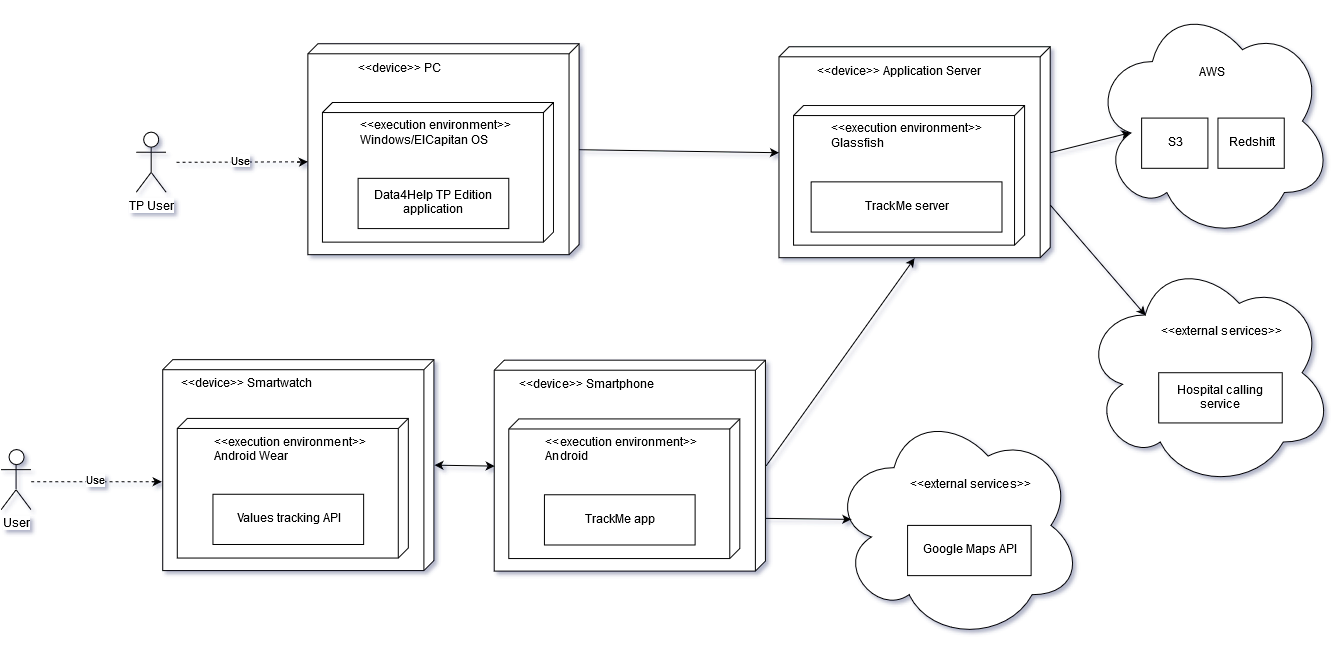
\includegraphics[width=\linewidth, keepaspectratio]{./Images/deployment_view.png}
    \centering
    \caption{Deployment View}
    \label{fig:depview}
  \end{figure}

\paragraph{} The deployment view shows the distribution of software and hardware in the TrackMe system. The components and their interactions are here described:
\begin{itemize}
\item{Data4Help TP Edition application} is the desktop application developed for third party users. This application makes queries and request to the Data4Help server, and receive updates of subcripted data, or various notification from Data4Help services.
\item TrackMe app is a general TrackMe app for smartphone: Data4Help, AutomatedSOS or Track4Run. Each one is able to connect to the TrackMe server, sending updates or managing operations according to the service, and is also able to receive updates and notifications from it. Track4Run must also be able to use Google Maps API in order to display the real time map during a competition.
\item Values tracking API: this is a generic smartwatch API which allows the TrackMe app to get data from the device, depending on which kind of device it is.
\item TrackMe Server is the core of the TrackMe environment, as it respond to most of the action performed by the users applications. In general, it receives a request from an application, determines the service and does the operation associated to it. Also for some kind of operation it communicates with the AWS services, or the ambulance calling service.
\item AWS is the chosen service for the DB deployment. All the accesses to it are made through the server, which stores Data4Help data on it, and also all the data used for the other two services.
\item The hospital calling service is the service defined with the D3 in the RASD (section 2.4). The calls directed to it are made only through the TrackMe server.
\end{itemize}